\chapter{Ensayos y resultados}

\label{Chapter4}

En este capítulo se detallan los ensayos realizados al sistema completo y los resultados obtenidos durante las pruebas de funcionamiento.

\section{Banco de pruebas}

El sistema consta físicamente de 2 tipos de componentes, nodos y servidor. El servidor posee a su vez la aplicación en el frontend y el backend con los módulos. También el sistema posee 2 tipos de nodos, control de calefacción y de iluminación.

Para ensayar el nodo de temperatura se utilizaron los materiales que lo componen que se muestran en la figura \ref{fig:30}.

\begin{figure}[h]
\centering
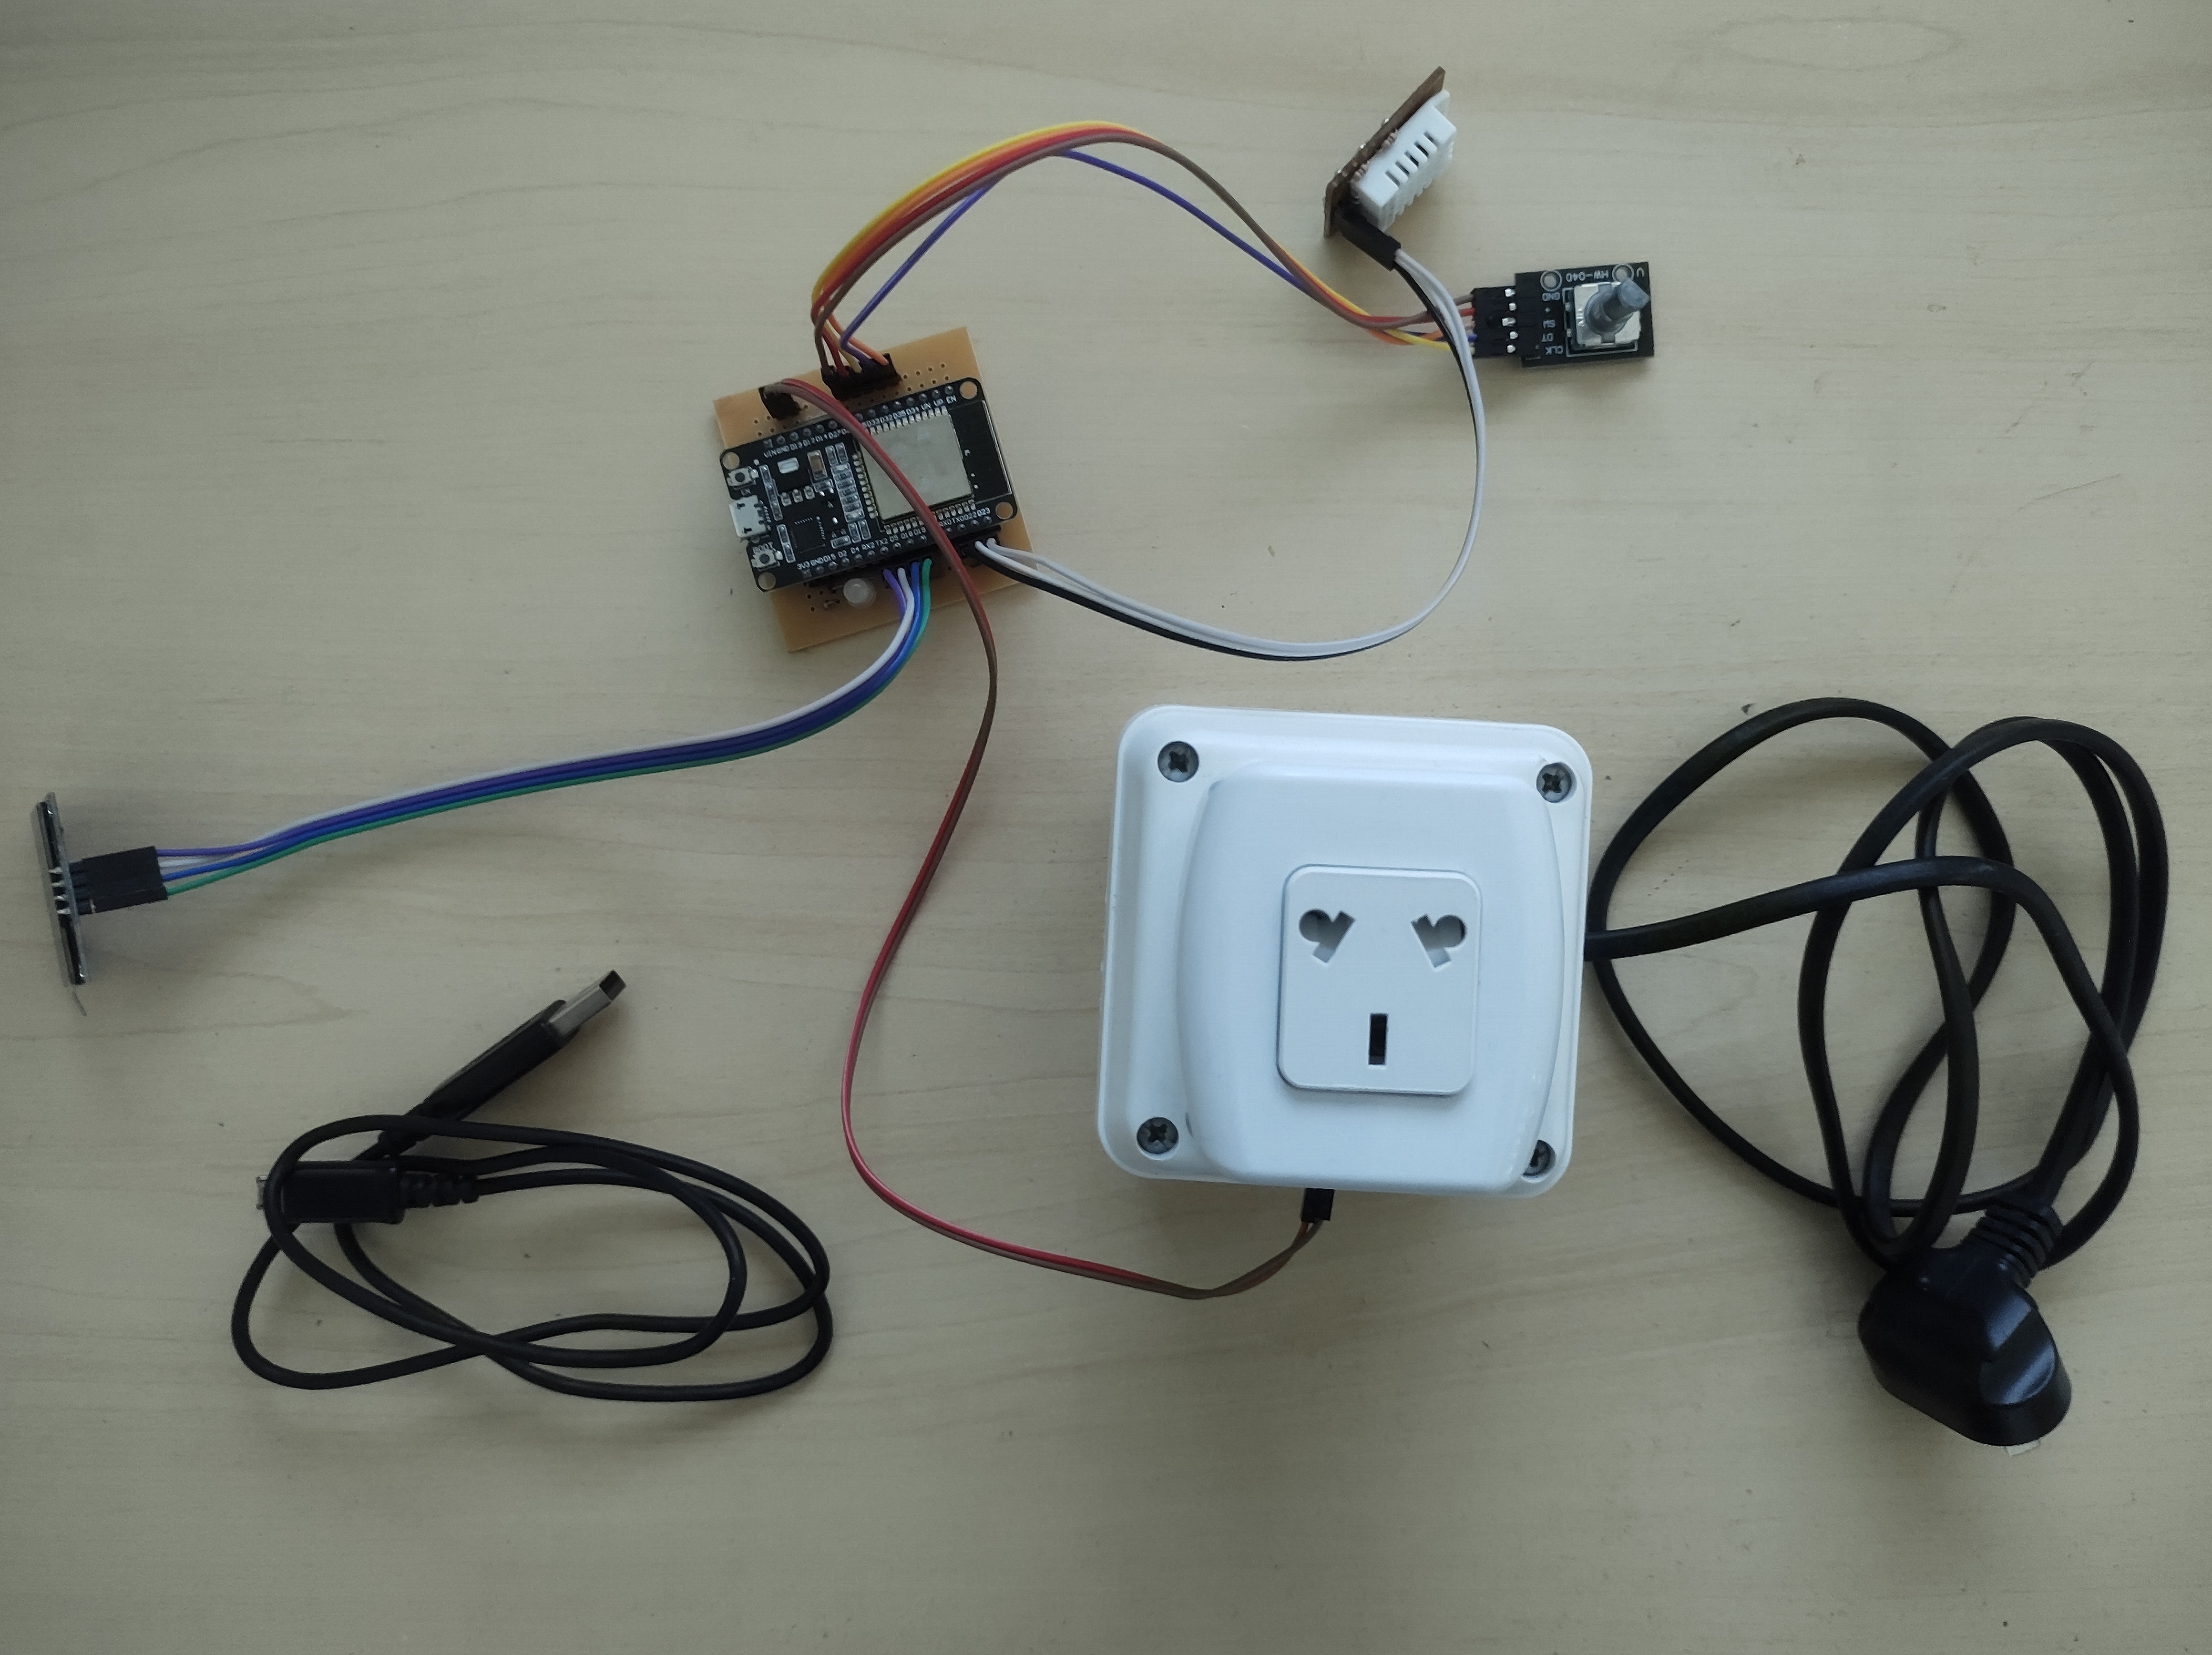
\includegraphics[scale=0.06]{Imagen 30 - Nodo temperatura.jpg}
\caption[Nodo temperatura]{Componentes del nodo de temperatura.}
\label{fig:30}
\end{figure}

Se puede observar la placa ESP32 montada sobre la placa de conexiones, el display, encoder, sensor de temperatura y una caja estanca con una conexión de toma corriente para conectar la estufa a encender. Esta caja además posee un cable para conectar a 220 VCA para alimentar la estufa y que funcione como un interruptor. Cabe aclarar que en modo automático el control de temperatura funciona con una histéresis de 1 grado, por lo que al setear la temperatura en un valor determinado, el control va a apagar la salida cuando la temperatura sobrepase por 1 grado al set-point y la va a encender cuando esté 1 grado por debajo de este valor.

Para ensayar el nodo de dimerización se utilizaron los materiales que lo componen que se muestran en la figura \ref{fig:31}.

\begin{figure}[h]
\centering
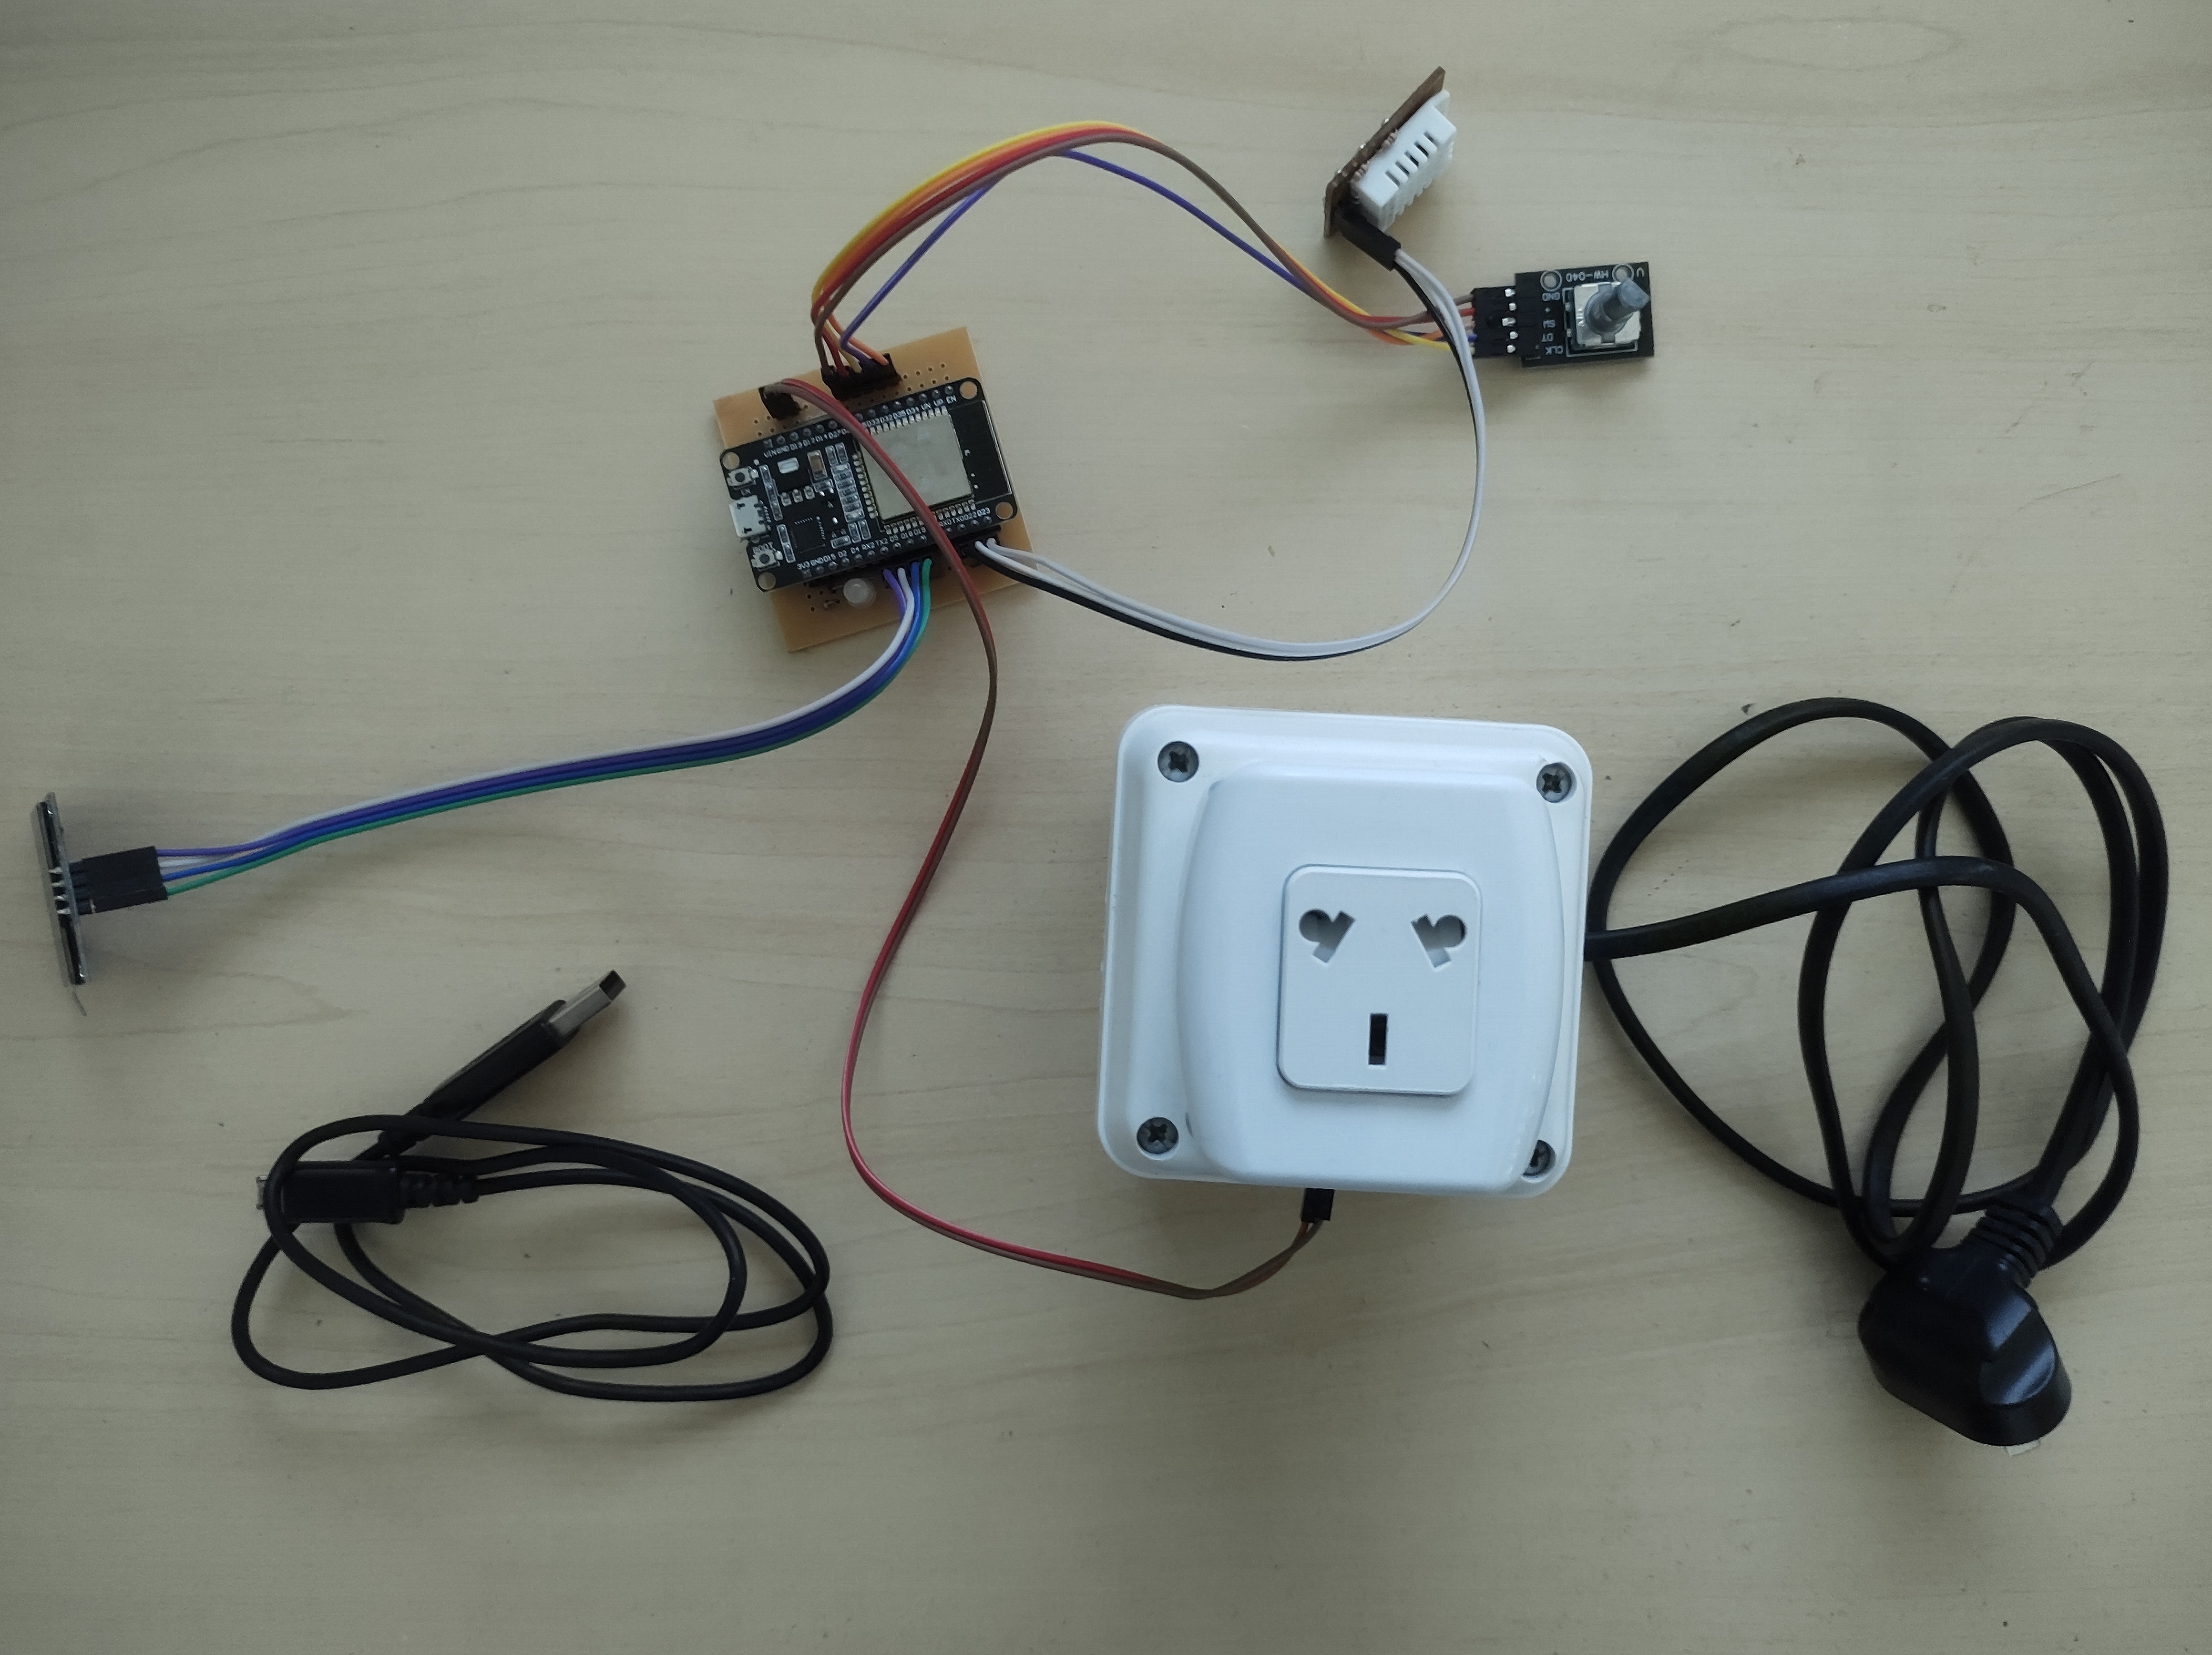
\includegraphics[scale=0.06]{Imagen 31 - Nodo dimmer.jpg}
\caption[Nodo dimmer]{Componentes del nodo de dimerización.}
\label{fig:31}
\end{figure}

Se puede observar la placa ESP32 montada sobre la placa de conexiones, el display, encoder, \textit{driver} de iluminación y la placa de LEDs de 5 VCC. El control posee un conector USB por lo que puede conectarse cualquier lámpara que funcione en este caso con 5 VCC y posea este conector.

En la figura \ref{fig:32} pueden verse los componentes que forman parte del servidor.

\begin{figure}[h]
\centering
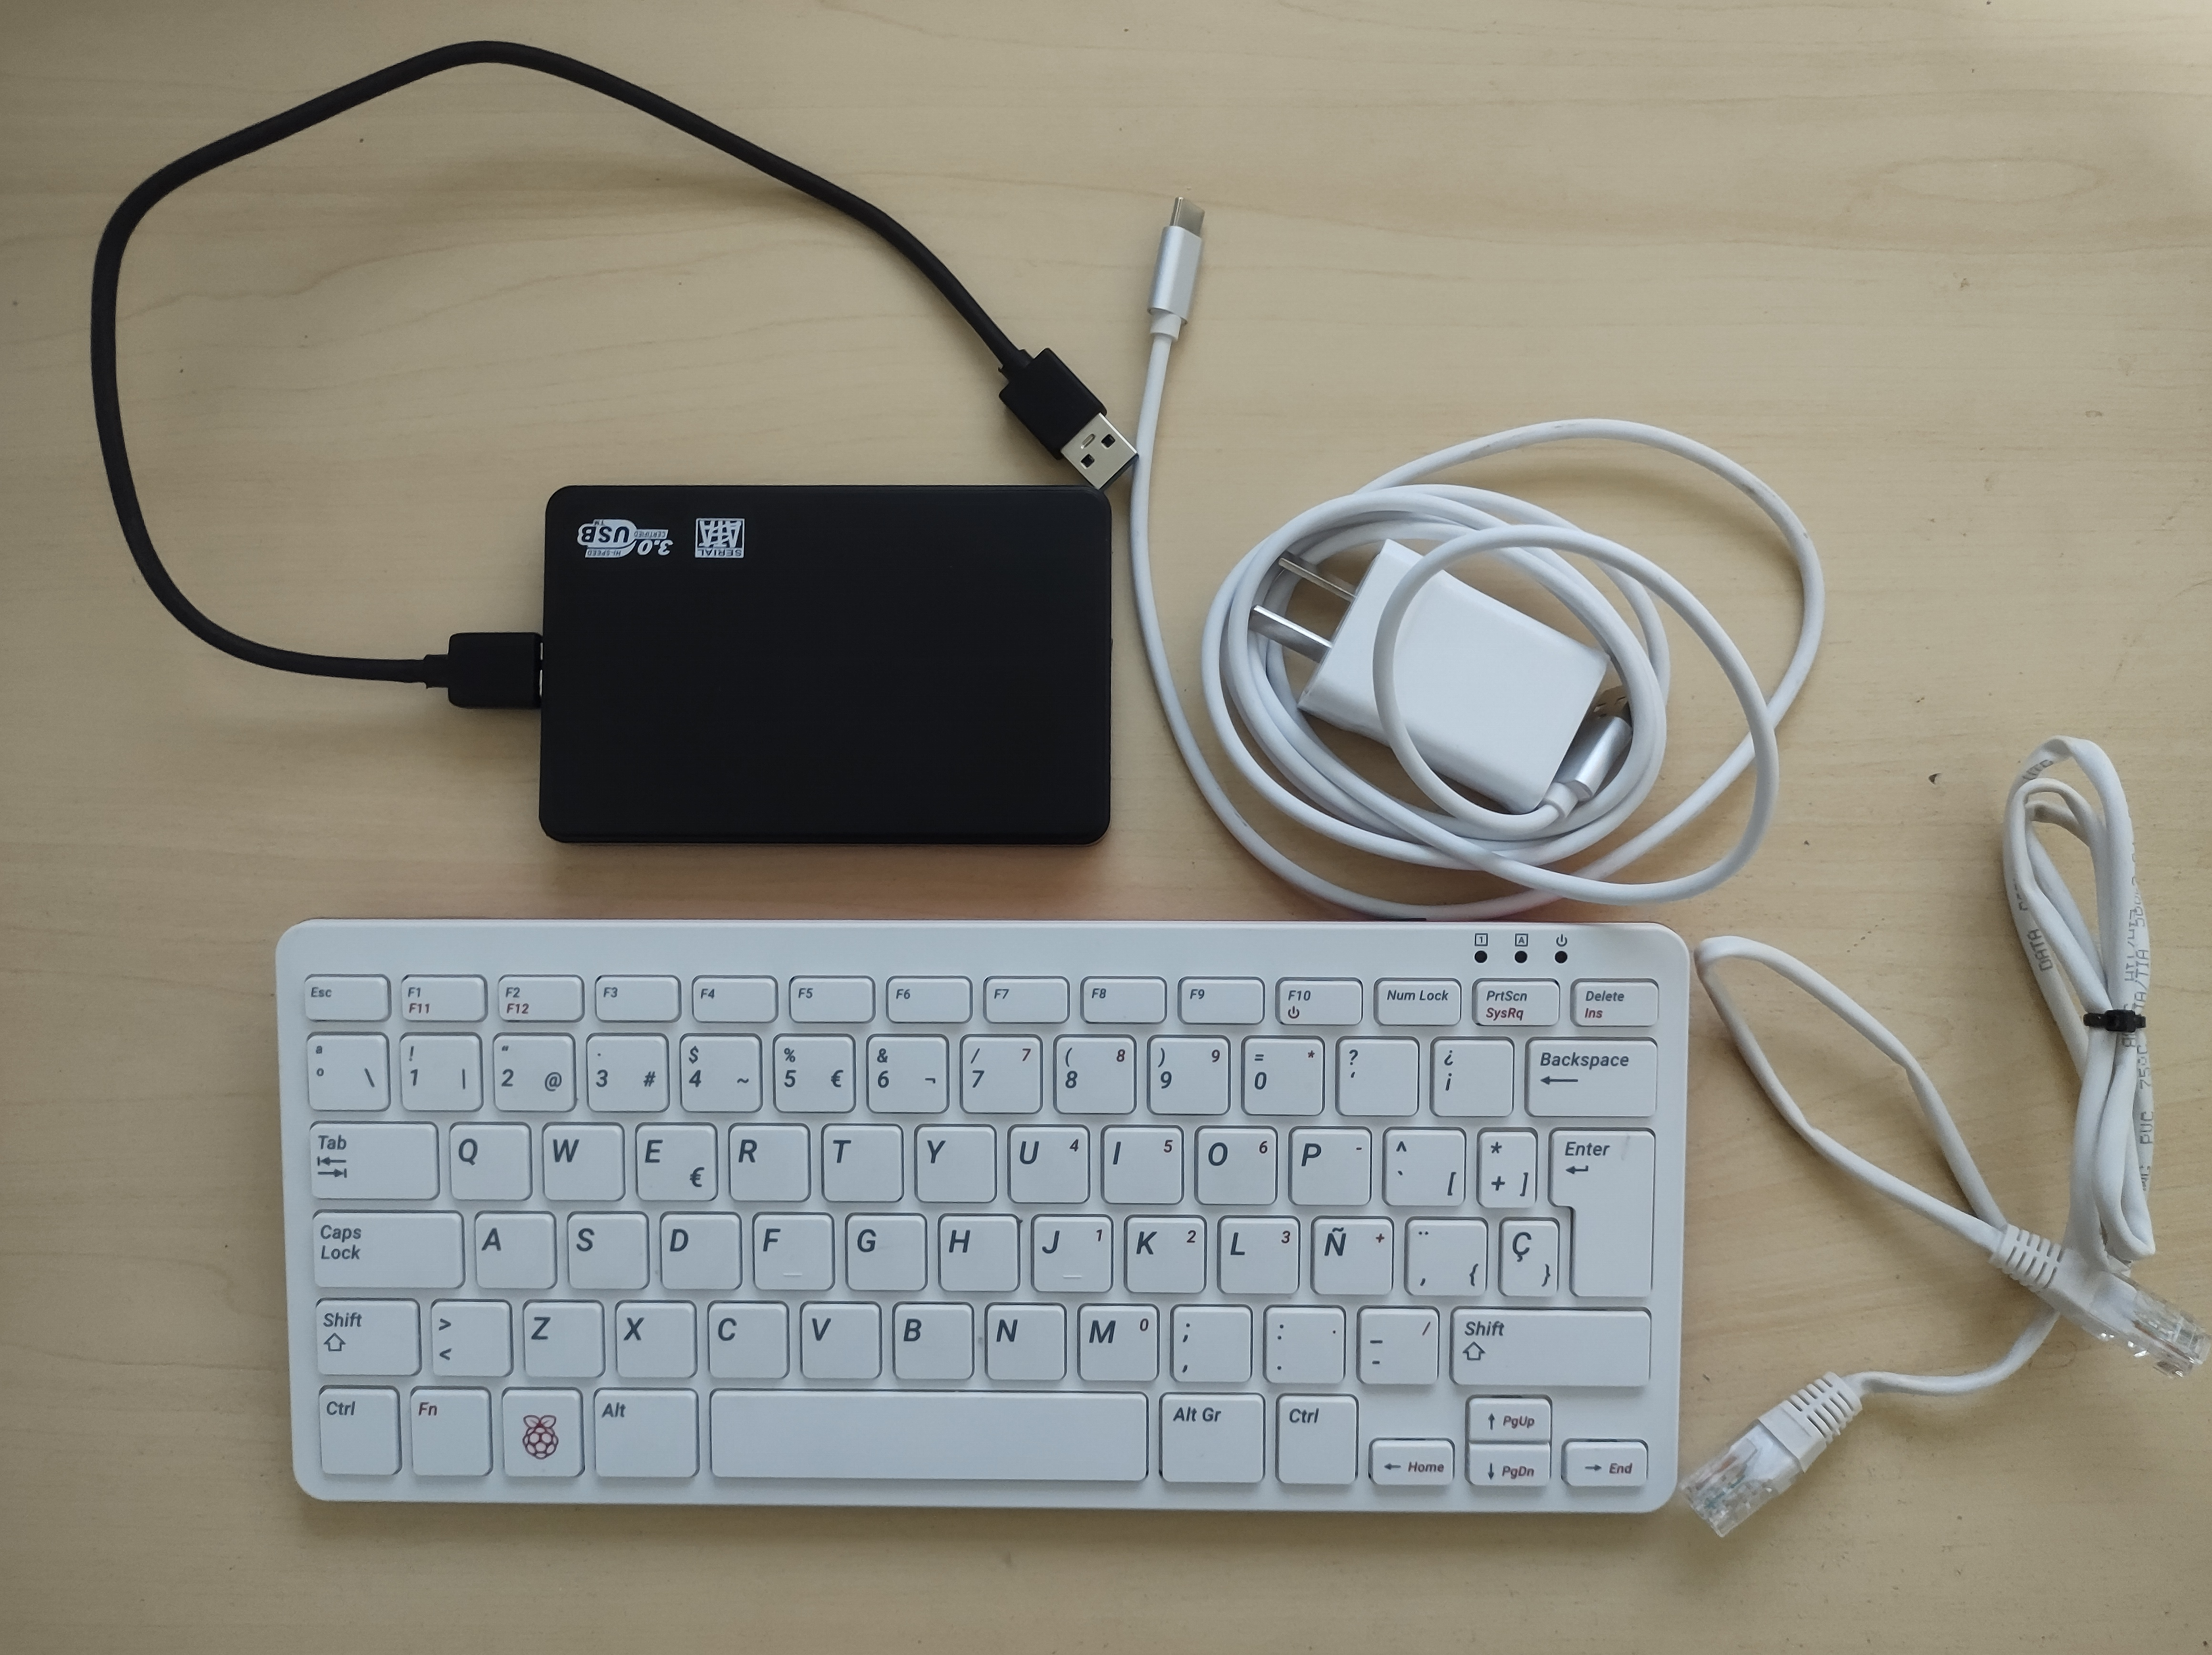
\includegraphics[scale=0.06]{Imagen 32 - Servidor.jpg}
\caption[Servidor]{Componentes del servidor.}
\label{fig:32}
\end{figure}

Puede observarse la Raspberry Pi400, la fuente de 5 VCC 3A con su cable, un disco rígido externo SSD de 120 GB y un cable Ethernet para la conexión a la red.

\section{Metodología empleada}

El hardware se testeó haciendo pruebas de funcionamiento con los materiales mostrados en la sección anterior. Las pruebas constaron de hacer funcionar los nodos por 2 días enteros corroborando que el control de temperatura funcione en los valores configurados y que la luminaria encienda y respete los valores de los saltos. Además se probó el funcionamiento de los horarios de encendido y apagado.

En cuanto al software se utilizaron distintas metodologías para la depuración de forma manual de los embebidos, el frontend y el backend. A continuación se describen cada una de ellas.

\subsection{Pruebas del frontend}

Para el frontend se utilizaron pruebas funcionales manuales con el sistema funcionando. Básicamente el desarrollo fue progresivo con trabajo en paralelo. Esto fue hacer una aplicación básica primero y luego seguir sumando funcionalidades. A medida que el sistema fue creciendo se fueron agregando más componentes hasta tener la versión actual.

Para las pruebas se utilizó la salida de la consola del navegador a medida que se iban implementando funciones y páginas nuevas. Con esto se logró mostrar en tiempo real el funcionamiento del sistema en cada una de las páginas y con cada función que se fue agregando. En el código \ref{lst:console front} se muestra a modo de ejemplo parte del desarrollo de la página para la visualización de un mensaje por consola de la configuración de un dispositivo.

\begin{lstlisting}[caption={Muestra por consola de los datos recibidos}, label={console front}]
ngOnInit() {
    const deviceId = this.activatedRoute.snapshot.paramMap.get('id') as string;
    this.dispositivoId = deviceId, 10;
    this.subscription = this.dispositivoService.getDeviceById(this.dispositivoId).subscribe((data) => {
      console.log(data);
      this.device = data[0];
      this.tipo = data[0].tipo;
      this.ubicacion = data[0].ubicacion;
    });
    this.leerdatos();
  }
\end{lstlisting}

Allí se puede ver la función \textit{console.log} mostrando los datos por consola. En la figura \ref{fig:33} se puede ver la pantalla de configuración del dispositivo y el mensaje por consola con los datos recibidos.

\begin{figure}[h]
\centering
\includegraphics[scale=0.4]{Imagen 33 - Consola front.png}
\caption[Prueba frontend]{Pantalla de aplicación y consola.}
\label{fig:33}
\end{figure}

Este mecanismo se utilizó en todas las páginas de la aplicación web y gracias a su utilización se consiguieron los resultados esperados de funcionalidad y errores.

\subsection{Pruebas del backend}

Para el backend se utilizó un mecanismo similar de pruebas funcionales que para el frontend.

El desarrollo fue progresivo por lo que a medida que se fueron incorporando funciones o endpoints nuevos, se fueron colocando muestras por consola para poder observar si los datos y las consultas estaban siendo resueltos de forma correcta. En el código \ref{lst:console back} se muestra como ejemplo el \textit{router} para borrar la tabla de mediciones de un dispositivo y el mensaje por consola de éxito y el ID del dispositivo.

\begin{lstlisting}[caption={Muestra por consola de los datos consultados}, label={console back}]
borrarTablaRouter.delete('/:id', async function (req, res, next) {
  const id = req.params.id;
  let connection;
  try {
      connection = await pool.getConnection();
      await connection.beginTransaction();
      const deleteMedicionesQuery = 'DELETE FROM Mediciones WHERE dispositivoId = ?';
      await connection.query(deleteMedicionesQuery, id);
      await connection.commit();
      connection.release();
      res.send({ message: 'Mediciones eliminadas exitosamente' }).status(200);
      console.log('Solicitud de eliminacion recibida para dispositivoId:', id);
      } catch (err) {
          if (connection) {
              await connection.rollback();
              connection.release();
          }
          res.send(err).status(400);
          console.log('Error al eliminar mediciones:', err);
      }
  });
\end{lstlisting}

En la figura \ref{fig:34} se puede ver la consola con el mensaje de éxito y el ID del dispositivo cuya tabla de mediciones fue eliminada.

\begin{figure}[h]
\centering
\includegraphics[scale=0.65]{Imagen 34 - Consola back.png}
\caption[Prueba backend]{Mensaje por consola del servidor.}
\label{fig:34}
\end{figure}

A estas pruebas se sumó el uso de la aplicación \textit{MQTTX} para testear la comunicación con el \textit{broker} y los dispositivos, especialmente cuando se implementaba la seguridad con los certificados SSL. De esta forma se ensayaron la primera conexión segura, la inserción de datos desde un dispositivo simulado, el envío de configuración desde la aplicación a los nodos y el mensaje de solicitud de configuración inicial de un nodo, entre otros.

En la figura \ref{fig:35} puede verse la configuración

\begin{figure}[h]
\centering
\includegraphics[scale=0.53]{Imagen 35 - MQTTX.png}
\caption[MQTTX]{Pantalla de MQTTX.}
\label{fig:35}
\end{figure}

\subsection{Pruebas de los nodos}

Las placas ESP32 tienen un depurador de software incorporado por lo que se colocaron funciones de muestra de

\section{Resultados finales}



\section{Comparación con el estado del arte}